\capitulo{4}{Metodología}
Los modelos y simulaciones que desarrollados a continuación tienen como finalidad representar de forma simplificada el comportamiento de ciertas enfermedades infecciosas mediante sistemas dinámicos deterministas. A partir de datos reales, se emplean distintos modelos epidemiológicos clásicos para estudiar su evolución en diferentes contextos.

Además, se incorporan modificaciones a algunos de estos modelos con el objetivo de evaluar el impacto de estrategias de control, siendo la vacunación la medida principal. La metodología empleada no solo busca describir la propagación de la enfermedad, sino también explorar posibles formas de mitigarla.

\section{Modelo SI}
El modelo SI es un modelo determinista simple que divide la población en susceptibles (S) e infectados (I). Asume que no hay recuperación, una vez infectado, el individuo permanece infectado de forma permanente. Útil para enfermedades crónicas o sin inmunidad.

\textbf{Supuestos del modelo}. La población total N es contante y homogénea, por lo que no se tienen en cuenta ni nacimientos ni muertes, ya sean por la enfermedad o por otras causas. Por lo tanto, la población susceptible más la infectada es la población total. No existe recuperación, los individuos infectados permanecen en este estado permanentemente. La transmisión de la enfermedad ocurre por contacto entre individuos susceptibles e infectados.

Se muestra una representación esquemática del modelo SI mediante el diagrama de flujo, como se ve en la figura \ref{fig:diagrama SI}.

\begin{figure}[H]
    \centering
    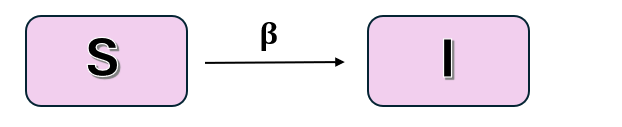
\includegraphics[width=0.7\textwidth]{img/diagrama_SI.png}
    \caption{Diagrama de flujo modelo SI}
    \label{fig:diagrama SI}
    \vspace{0.5cm} % Ajusta el espacio vertical entre la imagen y el texto
\end{figure}

También se puede describir el modelo a partir del siguiente sistema de ecuaciones diferenciales \ref{eq:ecuacion 1 Si}, \ref{eq:ecuacion 2 SI}.

\begin{align}
\frac{dS}{dt} &= -\beta SI \label{eq:ecuacion 1 Si} \\
\frac{dI}{dt} &= \beta SI \label{eq:ecuacion 2 SI}
\end{align}

Donde:
\begin{itemize}
    \item 	La ecuación dS⁄dt (\ref{eq:ecuacion 1 Si}), representa la variación del número de personas susceptibles a lo largo del tiempo. Como los individuos susceptibles se van infectando al entrar en contacto con personas contagiadas, este número disminuye progresivamente. Por esta razón, la derivada tiene signo negativo, expresa una pérdida en el grupo de los susceptibles debida al contagio.
    \item 	La ecuación dI⁄dt (\ref{eq:ecuacion 2 SI}), representa la variación del número de personas infectadas en el tiempo. Como los susceptibles que contraen la enfermedad pasan a formar parte del grupo de infectados, este valor aumenta a medida que progresa la transmisión, por lo que la derivada tiene signo positivo.
    \item El parámetro beta (~$\beta$) se denomina tasa de transmisión o de contagio. Representa la probabilidad de que un contacto entre un individuo susceptible y uno infectado resulte en un nuevo contagio. Es un valor clave en el modelo, ya que determina la velocidad con la que la enfermedad se propaga por la población. Como se muestra en la ecuación \ref{eq:beta} tiene unidades inversas al producto de personas y tiempo.
    \begin{equation}
    \beta = \frac{1}{\text{personas} \cdot \text{tiempo}}
    \label{eq:beta}
    \end{equation}
\end{itemize}

Hay que dejar claro que el modelo ha sido simplificado para su implementación en Simulink, se ha optado por no incluir explícitamente la población total. En su lugar, se redefine el parámetro beta, multiplicándolo por la población, incorporando de esta manera el efecto de la población total dentro del valor propio del parámetro. Esta modificación es algébricamente equivalente a la formulación original y permite mantener la coherencia del modelo al trabajar con cantidades absolutas de la población. 

La evolución del sistema a mediada que pasa el tiempo, el número de individuos susceptibles disminuye y el número de infectados crece. Como no existe la posibilidad de recuperación, la enfermedad termina por propagarse a toda la población.

Este modelo es interesante para enfermedades víricas crónicas, que causan infección de por vida y no tienen cura. Pueden ser algunas infecciones de transmisión sexual o ciertas condiciones virales persistentes. Sin embargo, la utilidad del modelo es limitada, ya que la mayoría de las enfermedades infecciosas contemplan la recuperación, lo cual no se refleja en este modelo.

El modelo se implementa en Simulink. Para mostrar su funcionamiento y lo que sería un resultado típico de este modelo, se realiza una simulación utilizando datos aleatorios, con el objetivo de observar el comportamiento del modelo SI en un caso práctico, se oberva en la figura \ref{fig:ejemplo SI}. Se considera una población total de 1000 individuos, con 999 personas susceptibles y 1 persona infectada al inicio. La tasa de transmisión utilizada es ~$\beta$ = 0.5. Sin embargo, dado que los valores de población con los que se trabajan son absolutos, esta tasa debe transformarse multiplicándola por la población total \ref{eq:betaefectiva}, resultando en un $\beta$ efectiva de 0.00005.
\begin{equation}
\beta_{\text{efectiva}} = \frac{\beta}{N} = \frac{0.05}{1000} = 0.00005
\label{eq:betaefectiva}
\end{equation}

Esto significa que, de media, cada persona infectada transmite la enfermedad al 0.005\% de la población susceptible por día.

\begin{figure}[H]
    \centering
    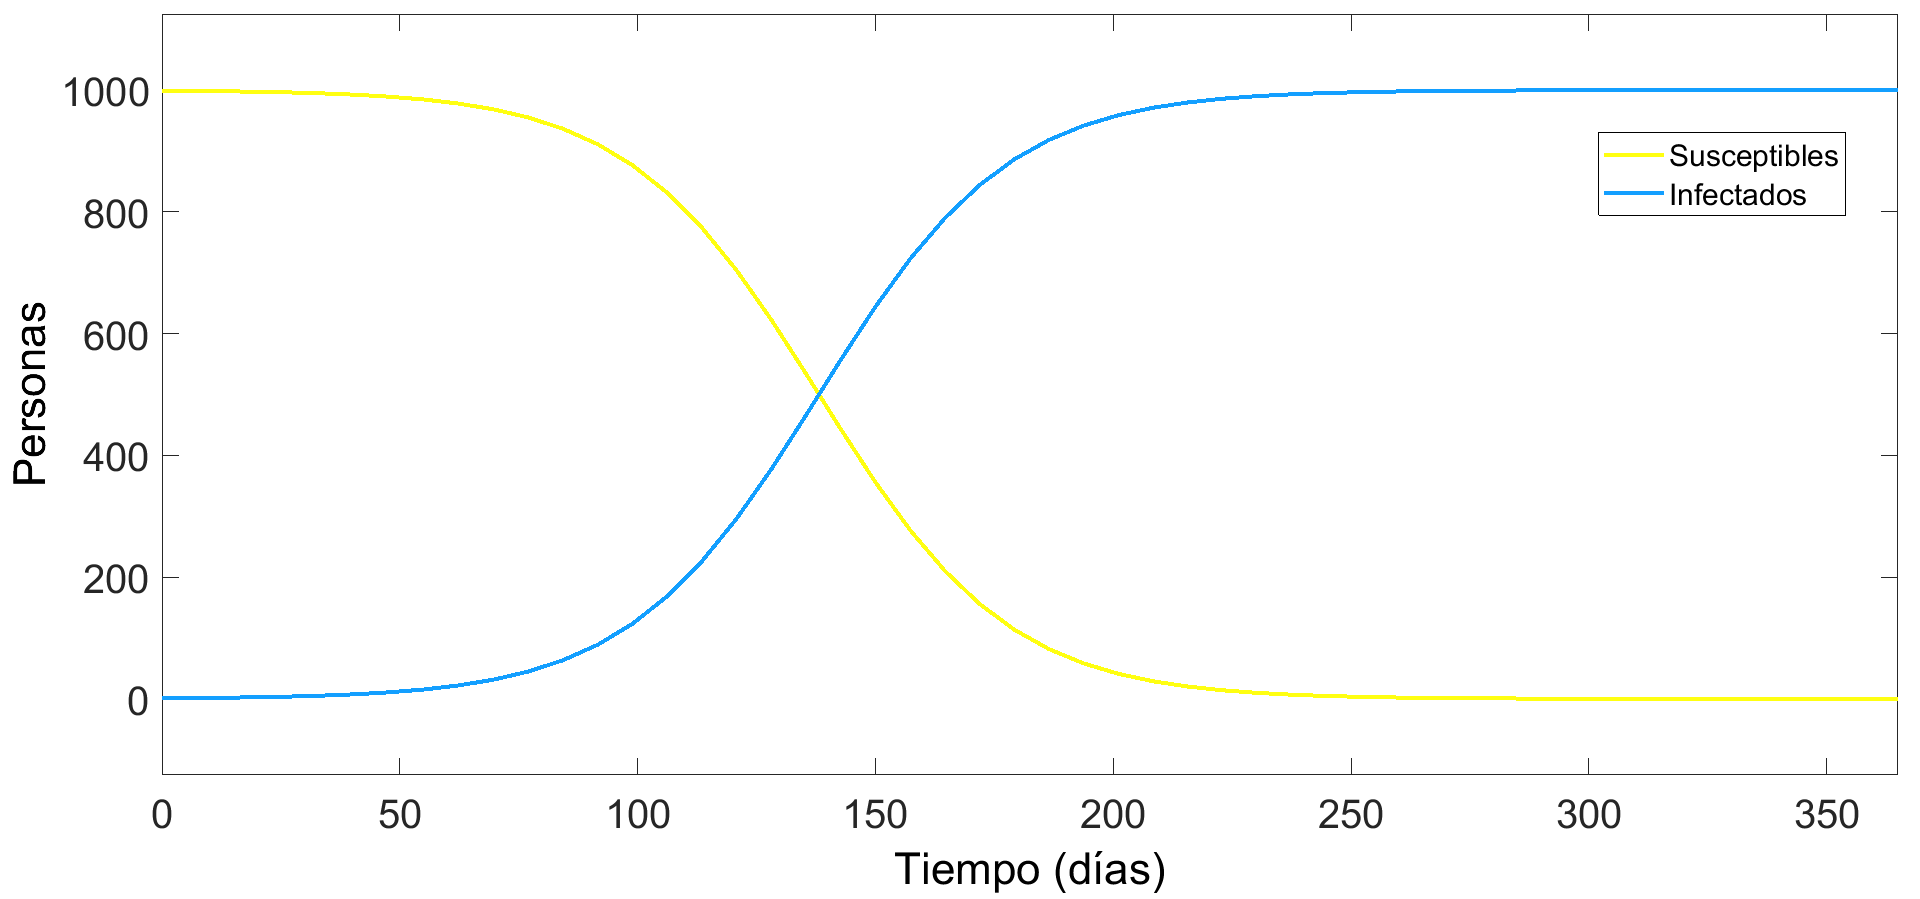
\includegraphics[width=0.7\textwidth]{img/modelo_SI_resultado_ejemplo.png}
    \caption{Resultado típico de un modelo SI}
    \label{fig:ejemplo SI}
    \vspace{0.5cm} % Ajusta el espacio vertical entre la imagen y el texto
\end{figure}

La evolución del modelo muestra una clara disminución en el número de personas susceptibles y un aumento en el número de infectados conforme pasa el tiempo. Inicialmente, casi toda la población es susceptible, lo que permite una propagación acelerada de la enfermedad, especialmente en las primeras etapas, debido a la alta probabilidad de contacto entre infectados y susceptibles.

La dinámica entre los susceptibles (S) y los infectados (I) está determinada por la tasa de transmisión $\beta$. Un valor alto de $\beta$ implica una propagación más rápida de la enfermedad, mientras que un $\beta$ bajo ralentiza el proceso.

En este modelo, que solo considera dos compartimentos S e I y no incluye recuperación, la enfermedad continúa propagándose hasta que toda la población ha sido infectada. Los infectados aumentan hasta que ya no quedan individuos susceptibles.


\section{Modelo SIS}
El modelo SIS representa enfermedades donde no se adquiere inmunidad tras la recuperación. Los individuos infectados se recuperan y vuelven a ser susceptibles, permitiendo reinfecciones. Es útil para estudiar enfermedades endémicas con contagio recurrente.

\textbf{Supuestos del modelo}. En este modelo también se asume que no ocurren ni nacimientos ni muertes, ya sean por la propia enfermedad o por otras circunstancias.

Se muestra una representación esquemática del modelo SIS mediante el diagrama de flujo, representado en la figura \ref{fig:diagrama SIS}.
\begin{figure}[H]
    \centering
    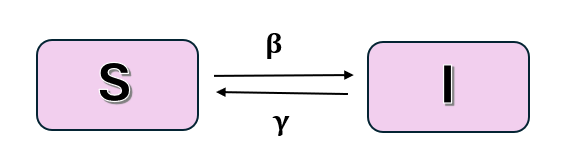
\includegraphics[width=0.7\textwidth]{img/diagrama_SIS.png}
    \caption{Diagrama de flujo modelo SIS}
    \label{fig:diagrama SIS}
    \vspace{0.5cm} % Ajusta el espacio vertical entre la imagen y el texto
\end{figure}

También se puede representar el modelo mediante el siguiente sistema de ecuaciones diferenciales \ref{eq:ec1SIS}, \ref{eq:ec2SIS}.

\begin{align}
\frac{dS}{dt} &= -\beta SI + \gamma I \label{eq:ec1SIS} \\
\frac{dI}{dt} &= \beta SI - \gamma I \label{eq:ec2SIS}
\end{align}

Donde:
\begin{itemize}
    \item 	La ecuación dS⁄dt (\ref{eq:ec1SIS}), representa la tasa de cambio de la población susceptible. Esta cantidad disminuye cuando los individuos se infectan, se expresa mediante un término negativo asociado a la tasa de contagio. Sin embargo, también aumenta cuando los individuos infectados se recuperan, ya que no se desarrolla inmunidad y vuelven a ser susceptibles. Por eso la tasa de recuperación aparece con signo positivo.
    \item 	La ecuación dI⁄dt (\ref{eq:ec2SIS}), representa la tasa de cambio de la población infectada. Este valor aumenta como consecuencia de los nuevos contagios, se refleja con término positivo asociado a la tasa de transmisión. A su vez, disminuye cuando los infectados se recuperan y regresan al compartimento de susceptibles, por ello gamma aparece con signo negativo.
    \item 	El parámetro beta ($\beta$) se denomina tasa de transmisión o de contagio. Representa la probabilidad de que un contacto entre un individuo susceptible y uno infectado resulte en un nuevo contagio. Es un valor clave en el modelo, ya que determina la velocidad con la que la enfermedad se propaga por la población. Las unidades de la tasa de transmisión, beta, siguen siendo las mismas, se ven en la ecuación \ref{eq:beta}.
    \item 	El parámetro gamma ($\gamma$) se denomina tasa de recuperación. Indica la probabilidad de que un individuo infectado se recupere y vuelva a ser susceptible, es este contexto. Las unidades de la tasa de recuperación gamma son \[[\text{tiempo}]^{-1}\] Que se pueden interpretar como el inverso del tiempo medio de recuperación \ref{eq:gammacal}.
    \begin{equation}
    \gamma = \frac{1}{\text{tiempo medio de recuperación}}
    \label{eq:gammacal}
    \end{equation}
\end{itemize}

Hay que dejar claro que el modelo ha sido simplificado para su implementación en Simulink, se ha optado por no incluir explícitamente en el coeficiente la población total. En su lugar, se redefine el parámetro beta, multiplicándolo por la población, incorporando de esta manera el efecto de la población total dentro del valor propio del parámetro. Esta modificación es algébricamente equivalente a la formulación original y permite mantener la coherencia del modelo al trabajar con cantidades absolutas de la población. 

El modelo se implementa en Simulink. Para mostrar su funcionamiento y lo que sería un resultado típico de este modelo, se realiza una simulación utilizando datos aleatorios, con el objetivo de observar el comportamiento del modelo SIS en un caso práctico, se observa en la figura \ref{fig:ejeSIS}. Se tiene una población total de 1000 personas, de las cuales 990 son susceptibles y 10 son infectados. La tasa de transmisión utilizada es $\beta$ = 0.3. Sin embargo, dado que los valores de población con los que se trabajan son absolutos, esta tasa debe transformarse multiplicándola por la población total \ref{eq:beta_}, resultando en una $\beta$ efectiva de 0.0003.

\begin{equation}
\beta_{\text{efectiva}} = \frac{\beta}{N} = \frac{0.3}{1000} = 0.0003
\label{eq:beta_}
\end{equation}

Esto significa que, de media, cada persona infectada transmite la enfermedad al 0.005\% de la población susceptible por día.

El tiempo de recuperación medio es de 10 días, por lo que hay que calcular la tasa de recuperación, gamma \eqref{eq:gamma_valor}.
\begin{equation}
\gamma = \frac{1}{\text{tiempo medio de recuperación}} = \frac{1}{10} = 0.1
\label{eq:gamma_valor}
\end{equation}

Esto significa que, de media, el 10\% de los individuos infectados se recupera cada día y vuelve al estado de susceptible, en este modelo SIS.


\begin{figure}[H]
    \centering
    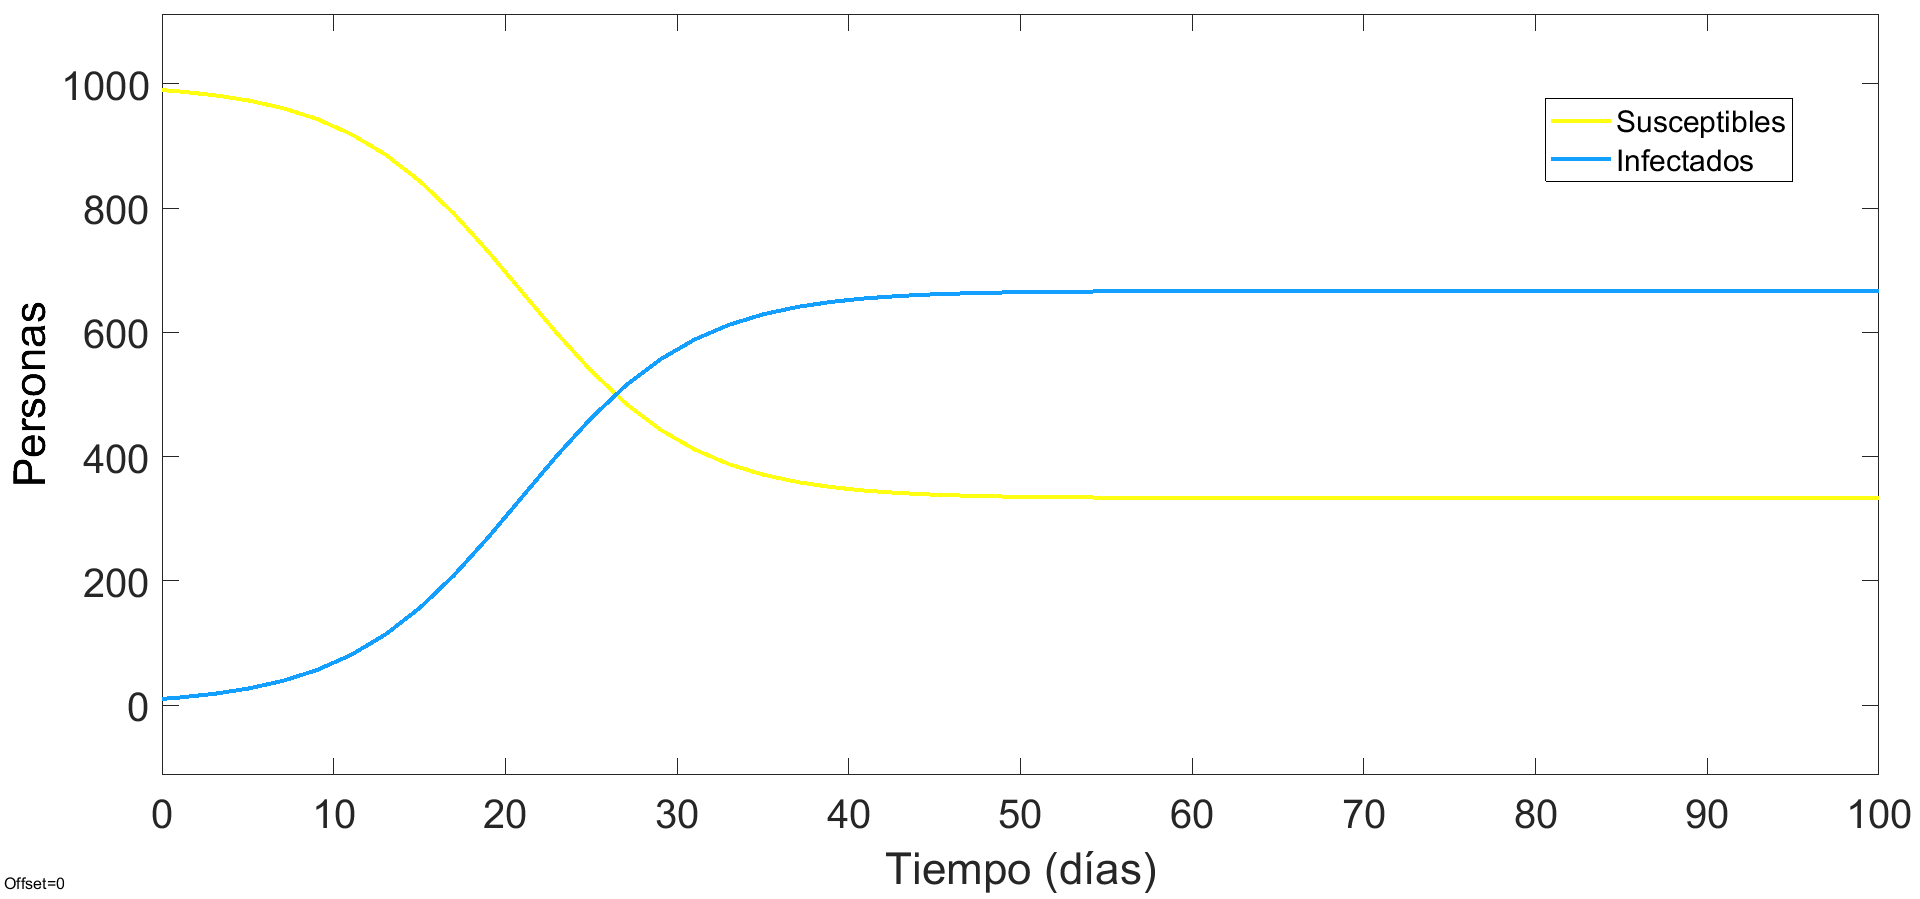
\includegraphics[width=0.7\textwidth]{img/modelo_SIS_resultado_ejemplo.png}
    \caption{Resultado típico de un modelo SIS}
    \label{fig:ejeSIS}
    \vspace{0.5cm} % Ajusta el espacio vertical entre la imagen y el texto
\end{figure}

La simulación de este modelo SIS, representada en la figura, muestra la evolución del número de individuos susceptibles e infectados a lo largo de 100 días. Partiendo de una población total, N, de 1000 personas.

En las primeras fases del brote, se observa un rápido incremento en el número de individuos infectados, acompañado de una disminución pronunciada en la población susceptible. Este comportamiento inicial se debe a la alta tasa de transmisión: hay numerosos contactos entre personas susceptibles e infectadas, lo que provoca una aceleración en el número de contagios.

Conforme avanza el tiempo, las curvas cambian sus pendientes: la velocidad de transmisión comienza a compensarse con la velocidad de recuperación, lo que da lugar a un punto de inflexión. A partir de ese momento, el sistema tiende hacia un estado de equilibrio epidemiológico, donde el número de nuevos contagios diarios es igual al número de recuperaciones. Esto se refleja en la estabilización de ambas curvas.

Este patrón es característico del modelo SIS, en el cual los individuos se recuperan, pero no adquieren inmunidad permanente, por lo que regresan al estado de susceptibles y pueden volver a infectarse. Como consecuencia, la enfermedad nunca desaparece completamente, sino que persiste en la población con un número constante de personas infectadas. Se alcanza así un equilibrio endémico, mantenido activa la enfermedad en ciertas poblaciones durante largos periodos.

Es importante calcular el número básico de reproducción \eqref{eq:R0_valor}, el cuál se va a explicar a continuación.
\begin{equation}
R_0 = \frac{\beta}{\gamma} = \frac{0.3}{0.1} = 3
\label{eq:R0_valor}
\end{equation}

Dado que $R_0$ = 3, por lo tanto, mayor que 1, la enfermedad se propaga y se mantiene en el tiempo. Este valor también explica el comportamiento observado en la gráfica, crecimiento inicial de los casos seguido de una estabilización, lo que confirma que el brte ha alcanzado un equilibrio endémico estable.




\subsection{Número básico de reproducción}
El comportamiento de un brote epidémico en los modelos compartimentales como el SIS está determinado, en gran parte, por un parámetro clave en epidemiología, el número básico de reproducción, representado como $R_0$.

Este parámetro se define como el número medio de infecciones secundarias que un solo individuo infectado es capaz de generar durante todo su periodo de infecciosidad, en una población compuesta exclusivamente por individuos susceptibles. Mide el potencial de propagación de la enfermedad en sus primeras etapas, antes de que otros factores como la inmunidad o la intervención sanitaria influyan en su dinámica.
El número básico de reproducción puede expresarse mediante la relación entre la tasa de transmisión y la de recuperación como se ve en la ecuación \ref{eq:ecR0}.

\begin{equation}
R_0 = \frac{\beta}{\gamma}
\label{eq:ecR0}
\end{equation}

Este coeficiente refleja el equilibrio entre la capacidad de la enfermedad para transmitirse y la velocidad con la que los individuos infectados se recuperan y regresan al estado de susceptibles. 
El valor de $R_0$ es fundamental para predecir la evolución del brote:
\begin{itemize}
    \item Si $R_0$ > 1, cada personas infectada contagia a más de una persona, lo que implica que la enfermedad se propaga y puede llegar a establecerse de forma endémica en la población.
    \item Si $R_0$ < 1, cada infectado genera, de media, menos de un caso nuevo, por lo que la enfermedad tiende a desaparecer con el tiempo.
    \item Si $R_0$ = 1, cada persona infectada reemplaza a otra, manteniendo el número de casos estable, pero sin expansión, no se produce un brote epidémico.
\end{itemize}
	
Cuando una enfermedad alcanza un valor de $R_0$ >1, pero sin provocar un crecimiento exponencial descontrolado, puede establecerse en un estado endémico. Esto significa que la enfermedad permanece presente de forma continua en una población o región determinada, con un número de casos que se mantiene relativamente constante a lo largo del tiempo.

La \textbf{endemicidad} implica que se ha alcanzado un equilibrio entre la transmisión del patógeno y los mecanismos que limitan su propagación, como, la inmunidad parcial de la población, la adaptación del agente patógeno a sus huéspedes y las intervenciones sanitarias o cambios de comportamiento.

Es importante aclarar que el hecho de que una enfermedad sea endémica no significa que sea benigna o que no represente un riesgo para la salud pública. De hecho, muchas enfermedades endémicas siguen teniendo un impacto considerable en términos de morbilidad y mortalidad, y requieren esfuerzos constantes de vigilancia, prevención y control.

\section{Modelo SIR}
El modelo SIR representa enfermedades donde los infectados se recuperan y adquieren inmunidad permanente. La población se divide en susceptibles, infectados y recuperados. Es útil para estudiar epidemias agudas y calcular el número básico de reproducción.

\textbf{Supuestos del modelo}. En este modelo se asume que la población total permanece constante, no hay nacimientos ni muertes. Los individuos solo pasan una sola vez por cada estado. La inmunidad es permanente durante el tiempo analizado. La mezcla entre individuos es homogénea, todos tienen la misma probabilidad de interactuar.
Aunque es un modelo idealizado, el SIR proporciona una herramienta potente para comprender y predecir el comportamiento de muchas enfermedades infecciosas, facilitando la toma de decisiones en salud pública y el diseño de estrategias de vacunación o contención.

Se muestra una representación esquemática del modelo SIS mediante el diagrama de flujo, representado en la figura \ref{fig:diagrama SIR}.
\begin{figure}[H]
    \centering
    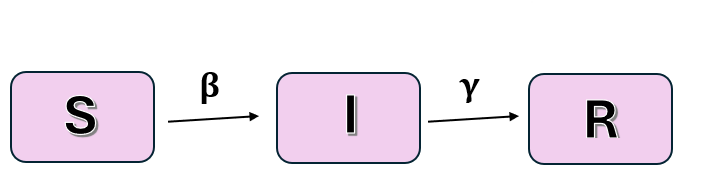
\includegraphics[width=0.7\textwidth]{img/diagrama_SIR.png}
    \caption{Diagrama de flujo modelo SIR}
    \label{fig:diagrama SIR}
    \vspace{0.5cm} % Ajusta el espacio vertical entre la imagen y el texto
\end{figure}

También se puede representar el modelo mediante el siguiente sistema de ecuaciones diferenciales \eqref{eq:ec1SIR}\eqref{eq:ec2SIR}\eqref{eq:ec3SIR}.

\begin{align}
\frac{dS}{dt} &= -\beta SI \label{eq:ec1SIR} \\
\frac{dI}{dt} &= \beta SI - \gamma I \label{eq:ec2SIR} \\
\frac{dR}{dt} &= \gamma I \label{eq:ec3SIR}
\end{align}

Donde:
\begin{itemize}
    \item 	La ecuación dS⁄dt \eqref{eq:ec1SIR}, explica la disminución de individuos susceptibles debido a nuevos contagios. Depende del número de susceptibles, de infectados y de la tasa de contacto efectivo. El signo es negativo ya que los susceptibles disminuyen con el tiempo.
    \item 	La ecuación dI⁄dt \eqref{eq:ec2SIR}, refleja los dos procesos que afectan a los infectados, el aumento de los nuevos contagios y la disminución por las recuperaciones. La diferencia entre estos dos términos determina si el número de infectados crece o disminuye.
    \item 	La ecuación dR⁄dt \eqref{eq:ec3SIR}, describe como aumenta el número de recuperados. 
    \item El parámetro beta ($\beta$) se denomina tasa de transmisión o de contagio. Representa la probabilidad de que un contacto entre un individuo susceptible y uno infectado resulte en un nuevo contagio. Es un valor clave en el modelo, ya que determina la velocidad con la que la enfermedad se propaga por la población. Las unidades de la tasa de transmisión beta se ven en la ecuación \eqref{eq:beta}.
    \item 	El parámetro gamma se denomina tasa de recuperación. Indica la probabilidad de que un individuo infectado se recupere y pase a recuperado, es este contexto. Se puede interpretar como el inverso del tiempo medio de recuperación, se calcula como en la ecuación \eqref{eq:gammacal}.
\end{itemize}

Hay que dejar claro que el modelo ha sido simplificado para su implementación en Simulink, se ha optado por no incluir explícitamente en el coeficiente la población total. En su lugar, se redefine el parámetro beta, multiplicándolo por la población, incorporando de esta manera el efecto de la población total dentro del valor propio del parámetro. Esta modificación es algébricamente equivalente a la formulación original y permite mantener la coherencia del modelo al trabajar con cantidades absolutas de la población. 

En cuanto al \textbf{número básico de reproducción $R_0$}, en el modelo SIR representa el promedio de personas susceptibles que una persona infectada puede contagiar durante todo el periodo que permanece infecciosa, en una población en la que todos los individuos son susceptibles al inicio del brote. Se calcula como ya se ha dicho anteriormente en la ecuación \eqref{eq:ecR0}

En este caso no es exactamente igual el significado dinámico entre el modelo SIS y el modelo SIR, aunque la fórmula es la misma. Se interpreta:
\begin{itemize}
    \item Si $R_0$ > 1: la enfermedad puede generar una epidemia, pero terminará desapareciendo cuando el número de susceptibles baje lo suficiente.
    \item Si $R_0$ < 1: la enfermedad no se propaga en la población y se extinguirá rápidamente.
\end{itemize}

Es clave en el modelo ya que permite predecir si una enfermedad se propagará o no, calcular el umbral de inmunidad necesario para detener la epidemia y guiar la implementación de estrategias de control. Por tanto, R0 no solo es un parámetro matemático, sino también una herramienta epidemiológica de gran valor.

El modelo se implementa en Simulink. Para mostrar su funcionamiento y lo que sería un resultado típico de este modelo, se realiza una simulación utilizando datos aleatorios, con el objetivo de observar el comportamiento del modelo SIR en un caso práctico, se oberva en la figura \ref{fig:ejemplo SIR}. La población total es de 10000, siendo susceptibles iniciales 9900 individuos, 100 individuos iniciales infectados y 0 individuos recuperados.
La tasa de transmisión utilizada es $\beta$ = 0.3. Sin embargo, dado que los valores de población con los que se trabajan son absolutos, esta tasa debe transformarse multiplicándola por la población total \eqref{eq:beta_efectiva_valor}, resultando en una beta efectiva de 0.00003.

\begin{equation}
\beta_{\text{efectiva}} = \frac{\beta}{N} = \frac{0.3}{10000} = 0.00003
\label{eq:beta_efectiva_valor}
\end{equation}

El tiempo de recuperación medio es de 5 días, por lo que hay que calcular la tasa de recuperación, gamma \eqref{eq:gamma_valor_dias}.

Significa que, de media, el 20\% de los individuos infectados se recupera cada día y se pasa al compartimento de los recuperados.

\begin{equation}
\gamma = \frac{1}{\text{tiempo medio de recuperación}} = \frac{1}{5} = 0.2\ \text{días}^{-1}
\label{eq:gamma_valor_dias}
\end{equation}


\begin{figure}[H]
    \centering
    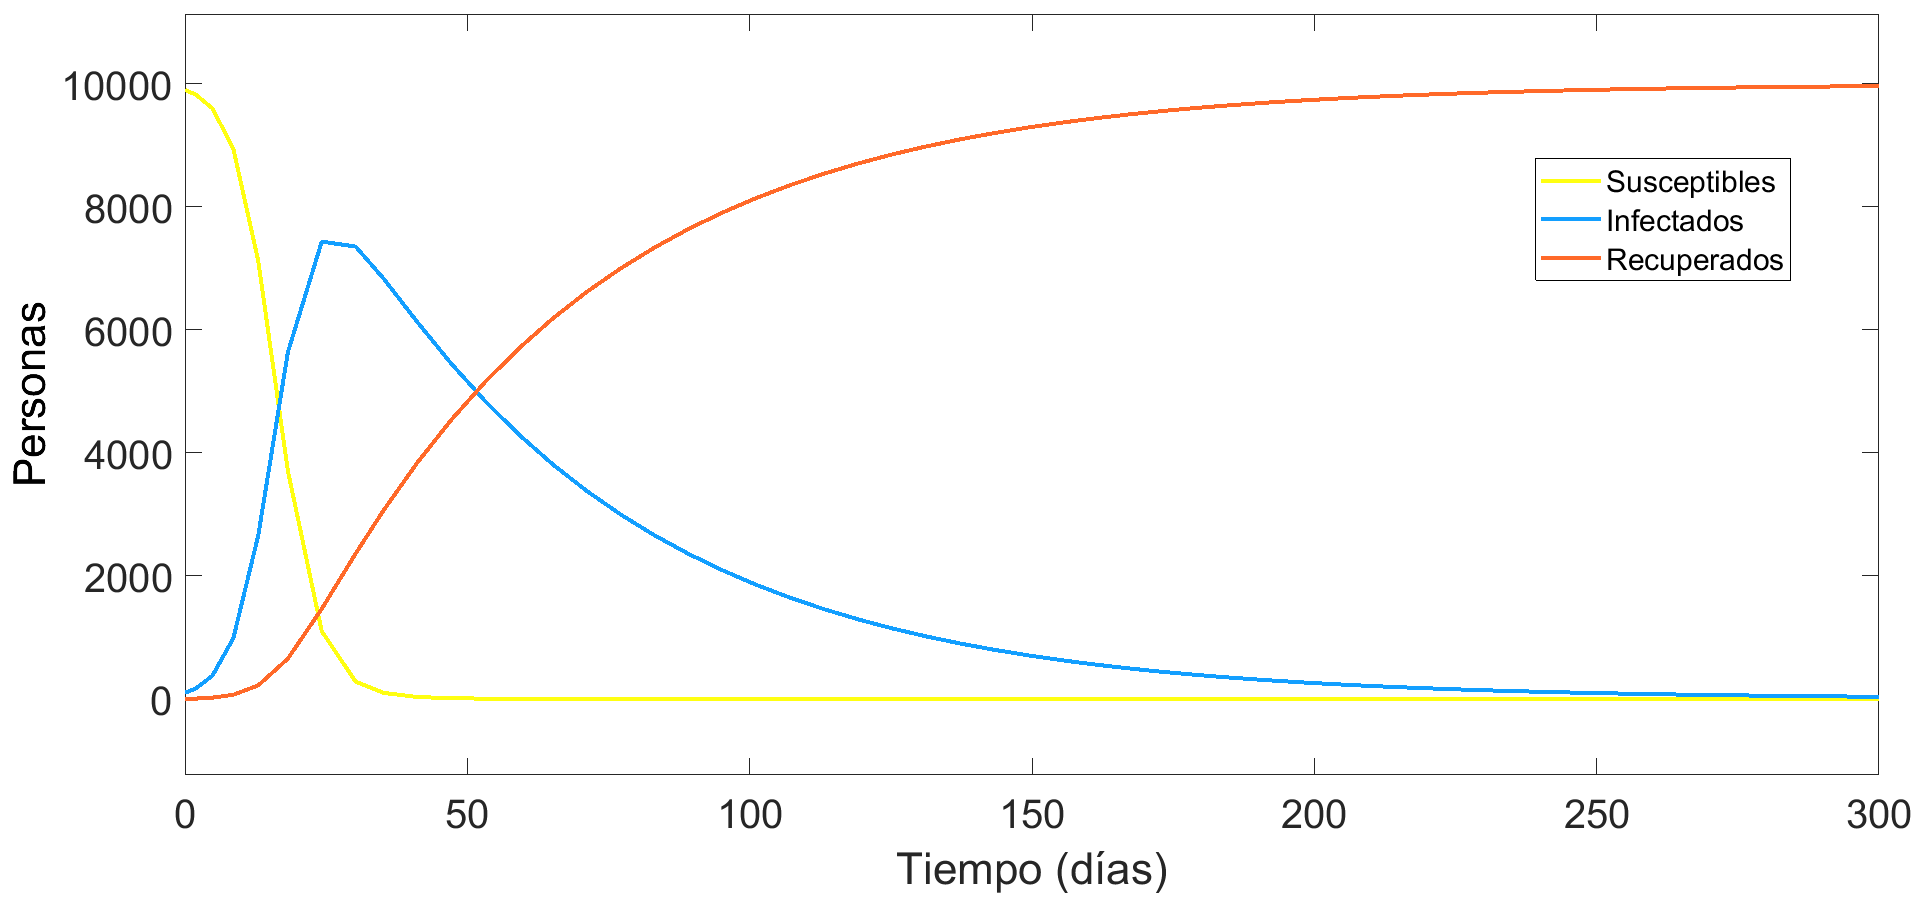
\includegraphics[width=0.7\textwidth]{img/modelo_SIR_resultado_ejemplo_.png}
    \caption{Resultado típico de un modelo SIR}
    \label{fig:ejemplo SIR}
    \vspace{0.5cm} % Ajusta el espacio vertical entre la imagen y el texto
\end{figure}


Al simular el modelo SIR durante un periodo de 300 días, se observa en la gráfica \ref{fig:ejemplo SIR} un comportamiento típico de una epidemia aguda, la enfermedad se propaga rápidamente, alcanza un pico epidémico y, finalmente, desaparece de la población.

Inicialmente, casi toda la población pertenece al compartimento de susceptibles. Desciende en los primeros días, debido a que una gran proporción de personas se infecta en un corto intervalo de tiempo. Esta rápida disminución refleja una enfermedad altamente contagiosa, que logra alcanzar a prácticamente toda la población susceptible.

El número de infectados crece de forma acelerada, alcanzando un máximo en el que se observa un gran número de personas enfermas a la vez. Sin embargo, a medida que estos infectados se recuperan y pasan al compartimento de recuperados, la curva de infectados comienza a descender, ya que quedan menos susceptibles disponibles para ser contagiados. El número de infectados tiende a cero.

La curva de recuperados comienza en cero y aumenta progresivamente, hasta que toda la población termina en este compartimento. Esto indica que, a largo plazo, todos los individuos se recuperan de la enfermedad y adquieren inmunidad, lo que impide que la infección vuelva a propagarse. La inmunidad permanente característica del modelo SIR es la que permite que la epidemia desaparezca de manera definitiva.

Se calcula el número básico de reproducción con estos parámetros\eqref{eq:R0_actualizado}.
\begin{equation}
R_0 = \frac{\beta}{\gamma} = \frac{0.3}{0.02} = 15
\label{eq:R0_actualizado}
\end{equation}

Este valor de $R_0$ es muy elevado, indica que cada personas infectada contagia, de media a 15 individuos,sería el caso de una enfermedad muy transmisible. La combinación de alta tasa de transmisión y tasa de recuperación relativamente baja favorece una propagación muy rápida, alcanzando una alta proporción de infectados al mismo tiempo. Esto lo podemos ver en el resultado de la figura \ref{fig:ejemplo SIR}.

Finalmente, al tratarse de un modelo SIR, los individuos que se recuperan no pueden volver a infectarse, a diferencia del modelo SIS, donde los recuperados retornan al grupo de susceptibles. Esta diferencia es clave para entender por qué, en este caso, la epidemia se extingue completamente una vez que se alcanza la in munidad de grupo, dejando a toda la población en el compartimento de recuperados.

\subsection{Mejora del modelo SIR}
Mejorar el modelo SIR como medida de control, incorporando explícitamente el efecto de la vacunación. Esta adaptación se conoce como modelo \textbf{SIRV} (Susceptibles – Infectados – Recuperados – Vacunados) y permite representar de forma más precisa la evolución de enfermedades infecciosas en poblaciones donde existen campañas de inmunización.

En el modelo SIRV, las personas susceptibles pueden infectarse al entrar en contacto con individuos contagiados, pero también tienen la opción de vacunarse como medida preventiva. Se asume que la vacunación confiere inmunidad completa y permanente, lo que implica que los individuos vacunados no pueden contraer la enfermedad ni transmitirla, y permanecen en ese estado de forma indefinida. De este modo, el grupo de vacunados actúa como una barrera adicional a la propagación del virus, reduciendo la proporción de personas susceptibles en la población y limitando la posibilidad de nuevos brotes.

Esta mejora del modelo permite analizar el impacto de diferentes tasas de vacunación sobre la evolución de la enfermedad y estudiar posibles estrategias de control. Además, ofrece una visión más ajustada a la situación actual, en la que la vacunación juega un papel fundamental en la protección individual y colectiva frente a enfermedades.

\textbf{Supuestos del modelo}. Es importante señalar que se mantienen los mismos supuestos básicos que en el modelo SIR. La única diferencia es la incorporación de la vacunación como medida de control de la enfermedad. En este modelo, se asume que las personas susceptibles que reciben la vacuna adquieren una inmunidad equivalente a la de quienes se han recuperado de la infección. Por ello, se considera que los individuos vacunados pasan directamente del compartimento de susceptibles al de recuperados, sin transitar por el estado de infectados.

Se muestra una representación esquemática del modelo SIS mediante el diagrama de flujo, representado en la figura \ref{fig:ejemplo SIRV}.

\begin{figure}[H]
    \centering
    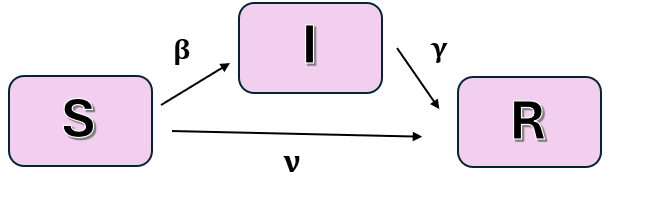
\includegraphics[width=0.7\textwidth]{img/diagrama_SIRV.png}
    \caption{Diagrma de flujo modelo SIRV}
    \label{fig:ejemplo SIRV}
    \vspace{0.5cm} % Ajusta el espacio vertical entre la imagen y el texto
\end{figure}

También se puede representar el modelo mediante el siguiente sistema de ecuaciones diferenciales \eqref{eq:ec1SIRV}\eqref{eq:ec2SIRV}\eqref{eq:ec3SIRV}.
\begin{align}
\frac{dS}{dt} &= -\beta SI - \nu S \label{eq:ec1SIRV} \\
\frac{dI}{dt} &= \beta SI - \gamma I \label{eq:ec2SIRV} \\
\frac{dR}{dt} &= \gamma I + \nu S \label{eq:ec3SIRV}
\end{align}

Donde:
\begin{itemize}
    \item 	La ecuación ds⁄dt \eqref{eq:ec1SIRV}, representa la disminución del número de personas susceptibles con el tiempo. Se reduce el número por dos mecanismos contagio y vacunación. Cuando los susceptibles entran en contacto con infectados, se contagian y dejan de ser susceptibles. Cuando los susceptibles se vacunan, también abandonan este estado. El signo negativo indica que la población susceptible disminuye con el tiempo.
    \item 	La ecuación dI⁄dt \eqref{eq:ec2SIRV}, describe la evolución del número de infectados. Aumenta por nuevos contagios y disminuye por recuperación. La diferencia entre los dos términos determina si el número de infectados crece generando un brote epidémico o decrece produciéndose un control de la enfermedad.
    \item 	La ecuación dR⁄dt \eqref{eq:ec3SIRV}, muestra como aumenta el número de personas inmunizadas. Se incluyen tanto a las personas recuperadas de la enfermedad como a los vacunados que pasan directamente al estado inmune. El crecimiento del comportamiento recuperado refleja la inmunidad de la población.
    \item 	Beta ($\beta$): tasa de transmisión o contagio, ya explicada anteriormente.
    \item 	Gamma ($\gamma$): tasa de recuperación, explicada anteriormente.
    \item	Nu ($\nu$): tasa de vacunación. Nuevo parámetro incluido que va a representar la fracción de la población susceptible que se vacuna por unidad de tiempo. Permite estudiar distintos escenarios de intervención sanitaria mediante campañas de vacunación. Sus unidades son
\[
[\text{tiempo}]^{-1}
\]
Se calcula como en la ecuación \eqref{eq:nu}
\begin{equation}
\nu = \frac{1}{\text{tiempo}}
\label{eq:nu}
\end{equation}
Es importante señalar, que normalmente lo que se encuentra es la cobertura de vacunación, por lo que hay que calcular la tasa de vacunación, para ello se utiliza la ecuación\eqref{eq:nu_log}.
\begin{equation}
\nu = \frac{-\ln(1 - \text{cobertura})}{\text{tiempo}}
\label{eq:nu_log}
\end{equation}


\end{itemize}

En este modelo no se ha incluido un compartimento explícito para los vacunados, ya que se asume que la vacunación proporciona una inmunidad equivalente a la adquirida tras pasar la enfermedad. Por lo tanto, las personas vacunadas son incorporadas de manera directa al compartimento de recuperados, simplificando así el modelo sin perder su capacidad explicativa. También dejar claro que no se añade la población total de forma explícita para su simplificación. Se redefine el parámetro beta como ya se ha visto anteriormente.

Es importante señalar que la tasa de transmisión ($\beta$) no varía directamente como consecuencia de la vacunación, ya que se trata de un parámetro biológico y social que describe la probabilidad de contagio efectivo entre un individuo susceptible y uno infectado por unidad de tiempo. Esta tasa depende de factores como la contagiosidad del virus, el número medio de contactos diarios entre personas y las medidas de comportamiento social.

Por tanto, $\beta$ se mantiene constante en el modelo si no cambian ni el virus ni las condiciones sociales de la población. Lo que sí se ve directamente afectado por la vacunación es el número de susceptibles. Al disminuir el tamaño del grupo susceptible mediante la inmunización, también se reduce la probabilidad de que se produzcan nuevos contagios, incluso si $\beta$ permanece constante. Aunque el virus mantenga su capacidad de contagio, al haber menos personas expuestas, disminuye el número efectivo de nuevas infecciones.

Además, se está utilizando la $\beta$ efectiva o ajustada, que es el valor de $\beta$ dividido entre la población total. En este caso, si la población total cambia, el valor de $\beta$ ajustada también cambiará, incluso si $\beta$ se mantiene constante. Esto se debe a que el tamaño poblacional afecta directamente al cálculo del número esperado de contactos efectivos entre susceptibles e infectados.

\subsection{Control PID para modelo SIR}
Con el objetivo de limitar la cantidad de personas infectadas, se incorporó un mecanismo de control basado en un regulador PID. Este controlador actúa modificando el parámetro $\beta$, lo que equivale a simular la implementación de medidas como el distanciamiento social, el confinamiento o el uso de mascarillas. El propósito del controlador es mantener el número de infectados cerca de un valor deseado, también llamado setpoint.

Las simulaciones se realizaron directamente en MATLAB, utilizando código para resolver numéricamente el sistema de ecuaciones diferenciales mediante el método de Euler. El controlador PID también se programó en MATLAB, permitiendo ajustar sus parámetros y analizar la respuesta del sistema en distintos escenarios, variando los valores de $\beta$ y $\gamma$. Esto permite observar el comportamiento de la epidemia y la capacidad del controlador para mantenerla bajo control.

En la figura \ref{fig:simu3pid} se muestra un ejemplo de la introducción de un regulador en el modelo. Se puede observar que el pico de infectados no alcanza un valor muy elevado, ya que el número de personas infectadas se mantiene aproximadamente en torno al valor de referencia (setpoint). A medida que la epidemia avanza y disminuye la cantidad de personas susceptibles, el número de infectados tiende a cero.
\begin{figure}[H]
    \centering
    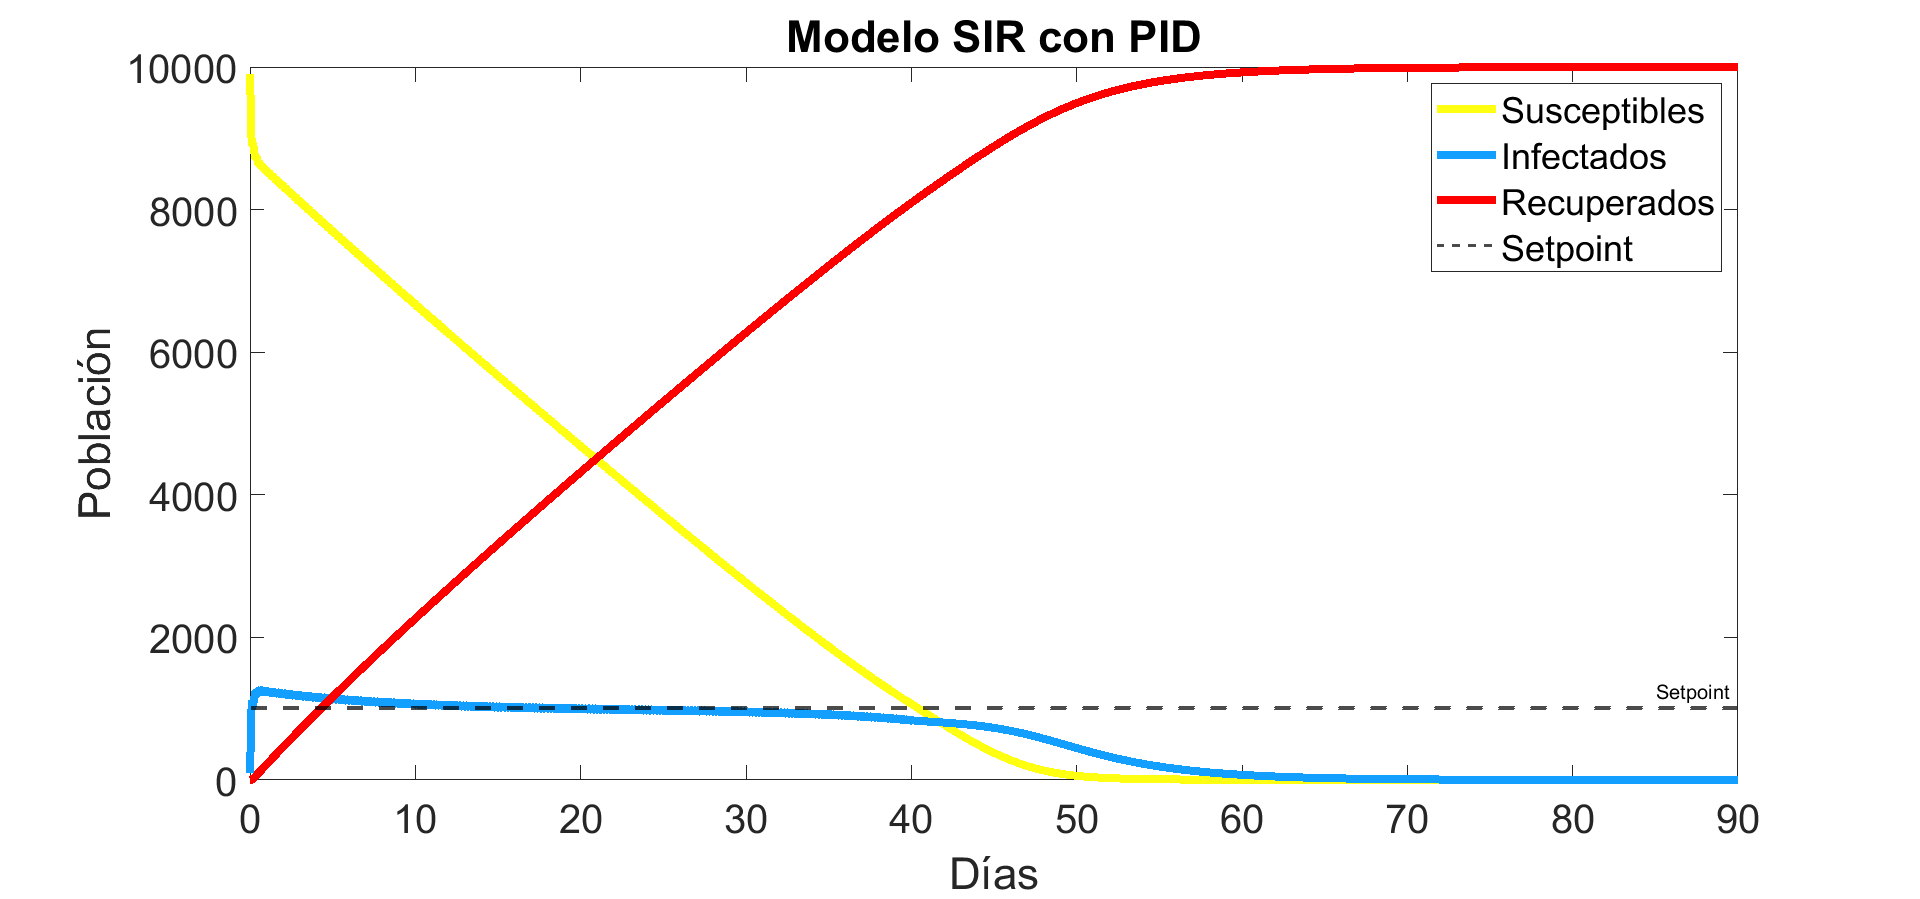
\includegraphics[width=0.7\textwidth]{img/modeloSIR_PID3.png}
    \caption{Simulación 1 para modelo SIR con PID}
    \label{fig:simu3pid}
    \vspace{0.5cm} % Ajusta el espacio vertical entre la imagen y el texto
\end{figure}

\section{Modelo SEIR}
El modelo SEIR añade un estado de exposición (E) al SIR, para representar enfermedades con periodo de incubación. Los individuos pasan de susceptibles a expuestos, luego a infectados y finalmente a recuperados con inmunidad. Es útil para modelar infecciones con retraso en la transmisibilidad.

\textbf{Suposiciones del modelo}. En este modelo se asume también que la población total es constante, sin nacimientos ni muertes, y que los individuos solo atraviesan una vez cada uno de los estados. Asimismo, se supone una mezcla homogénea, es decir, todos los individuos tienen la misma probabilidad de interactuar entre sí.

Relevante cuando se necesita considerar el impacto del periodo de incubación en la propagación de la enfermedad. Simplificación de la realidad, ofrece una aproximación más ajustada que el modelo SIR para muchas infecciones reales.

Se muestra una representación esquemática del modelo SIS mediante el diagrama de flujo, representado en la figura \ref{fig:diagrama SEIR}.
\begin{figure}[H]
    \centering
    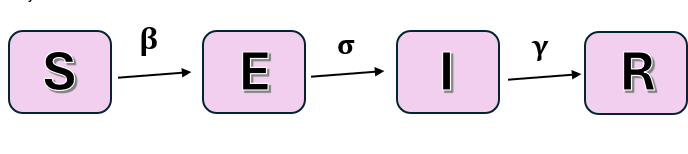
\includegraphics[width=0.7\textwidth]{img/diagrama_SEIR.png}
    \caption{Diagrma de flujo modelo SEIR}
    \label{fig:diagrama SEIR}
    \vspace{0.5cm} % Ajusta el espacio vertical entre la imagen y el texto
\end{figure}

También se puede representar el modelo mediante el siguiente sistema de ecuaciones diferenciales \eqref{eq:dS_SEIR}\eqref{eq:dE_SEIR}\eqref{eq:dI_SEIR}\eqref{eq:dR_SEIR}. 
\begin{align}
\frac{dS}{dt} &= -\beta SI \label{eq:dS_SEIR} \\
\frac{dE}{dt} &= \beta SI - \sigma E \label{eq:dE_SEIR} \\
\frac{dI}{dt} &= \sigma E - \gamma I \label{eq:dI_SEIR} \\
\frac{dR}{dt} &= \gamma I \label{eq:dR_SEIR}
\end{align}

Donde:
\begin{itemize}
    \item 	La ecuación dS⁄dt \eqref{eq:dS_SEIR}, representa la disminución de individuos susceptibles por el contacto con personas infectadas. La disminución depende del número de susceptibles, del número de infectados y de la tasa de transmisión. Es negativa porque los susceptibles disminuyen con el tiempo al contagiarse.
    \item 	La ecuación dE⁄dt \eqref{eq:dE_SEIR}, describe el cambio en el número de individuos expuestos. Aumenta cuando un susceptible se infecta y disminuye cuando uno expuesto pasa a la fase infecciosa.
    \item 	La ecuación dI⁄dt \eqref{eq:dI_SEIR}, muestra la evolución de los infectados. Aumenta cuando los expuestos se vuelven contagiosos y disminuye por las recuperaciones. El balance entre estos dos procesos determina si el número de infectados crece o decrece.
    \item 	La ecuación dR⁄dt \eqref{eq:dR_SEIR}, refleja el aumento de individuos recuperados, que ya no pueden contagiarse ni contagiar. La velocidad de recuperación está determinada por la tasa de recuperación.
    \item Beta ($\beta$), tasa de transmisión: representa la probabilidad de que un individuo susceptible se infecte tras entrar en contacto con un infectado. 
    \item Sigma ($\sigma$), tasa de incubación: la inversa del tiempo medio que tarda un individuo expuesto en volverse contagioso. Se calcula como en la ecuación \eqref{eq:sigma}.
    \begin{equation}
    \sigma = \frac{1}{\text{tiempo de incubación}}
    \label{eq:sigma}
    \end{equation}
    \item Gamma ($\gamma$), tasa de recuperación: indica cuántos infectados se recuperan por unidad de tiempo. Es el inverso del tiempo medio de infección.
\end{itemize}

\textbf{El número básico de reproducción $R_0$} sigue siendo importante ya que es un indicador clave para poder estimar el potencial de propagación de una enfermedad. Se calcula de la misma manera, como en la ecuación \eqref{eq:ecR0}. Determina si se producirá un brote:
\begin{itemize}
    \item 	Si $R_0$ > 1, la infección tiende a propagarse.
    \item 	Si $R_0$ <1, tiende a desaparecer.
\end{itemize}

Hay que dejar claro que el modelo ha sido simplificado para su implementación en Simulink, se ha optado por no incluir explícitamente en el coeficiente la población total. En su lugar, se redefine el parámetro beta, multiplicándolo por la población, incorporando de esta manera el efecto de la población total dentro del valor propio del parámetro. Esta modificación es algébricamente equivalente a la formulación original y permite mantener la coherencia del modelo al trabajar con cantidades absolutas de la población. 

Es importante tener en cuenta la distinción entre individuos infectados e infecciosos, especialmente al comparar diferentes modelos epidemiológicos. En los modelos SIR y SIS se asume que un individuo infectado pasa inmediatamente a ser infeccioso, que puede transmitir la enfermedad en el mismo instante en que se contagia. En estos modelos no se contempla un periodo de latencia.

Sin embargo, el modelo SEIR introduce una mejora al incorporar un compartimento de individuos expuestos. En este caso, cuando una persona susceptible entra en contacto con un individuo infeccioso, pasa primero al estado de “expuesto”, lo que significa que está infectada pero aún no es capaz de contagiar a otros. Este periodo de latencia representa el tiempo de incubación del patógeno, durante el cual el individuo no presenta síntomas y no es detectable clínicamente ni contagioso.

Este aspecto tiene implicaciones relevantes al momento de establecer las condiciones iniciales para una simulación. En la práctica, no es posible conocer con exactitud cuántas personas se encuentran en el estado de exposición, ya que no presentan síntomas, no dan positivo en pruebas diagnósticas inmediatamente y además tampoco tienen capacidad de contagiar.
Por esta razón, se va a asumir que el número inicial de expuestos es cero en las simulaciones. Aun así, este compartimento resulta fundamental para modelar de forma más realista enfermedades que incluyen un periodo de incubación significativo.


El modelo se implementa en Simulink. Para mostrar su funcionamiento y lo que sería un resultado típico de este modelo, se realiza una simulación utilizando datos aleatorios, con el objetivo de observar el comportamiento del modelo SEIR en un caso práctico \ref{fig:eje SEIR}. La población total es de 1000, siendo susceptibles iniciales 990 individuos, 10 individuos iniciales infectados y tanto expuestos como recuperados 0 individuos.
La tasa de transmisión utilizada es $\beta$ = 0.5. Sin embargo, dado que los valores de población con los que se trabajan son absolutos, esta tasa debe transformarse multiplicándola por la población total \eqref{eq:beta_efectiva_0.0005}, resultando en una beta efectiva de 0.0005.
\begin{equation}
\beta_{\text{efectiva}} = \frac{\beta}{N} = \frac{0.5}{1000} = 0.0005
\label{eq:beta_efectiva_0.0005}
\end{equation}
Por lo que una personas infectada contagia al 0.05\% de la población susceptible por día.
El tiempo de recuperación medio es de 14 días, por lo que hay que calcular la tasa de recuperación gamma \eqref{eq:gamma_77}.
\begin{equation}
\gamma = \frac{1}{\text{tiempo medio de recuperación}} = \frac{1}{14} = 0.071\ \text{días}^{-1}
\label{eq:gamma_77}
\end{equation}
Esto significa que, de media, el 7,1\% de los individuos infectados se recupera cada día y se pasa al compartimento de los recuperados.
En cuanto al tiempo de incubación es de 5,2 los individuos tardan este tiempo en ser contagiosos tras haberse infectado, por lo que hay que calcular la tasa de incubación \eqref{eq:sigma_valor}.
\begin{equation}
\sigma = \frac{1}{\text{tiempo de incubación}} = \frac{1}{5.2} \approx 0.19
\label{eq:sigma_valor}
\end{equation}

\begin{figure}[H]
    \centering
    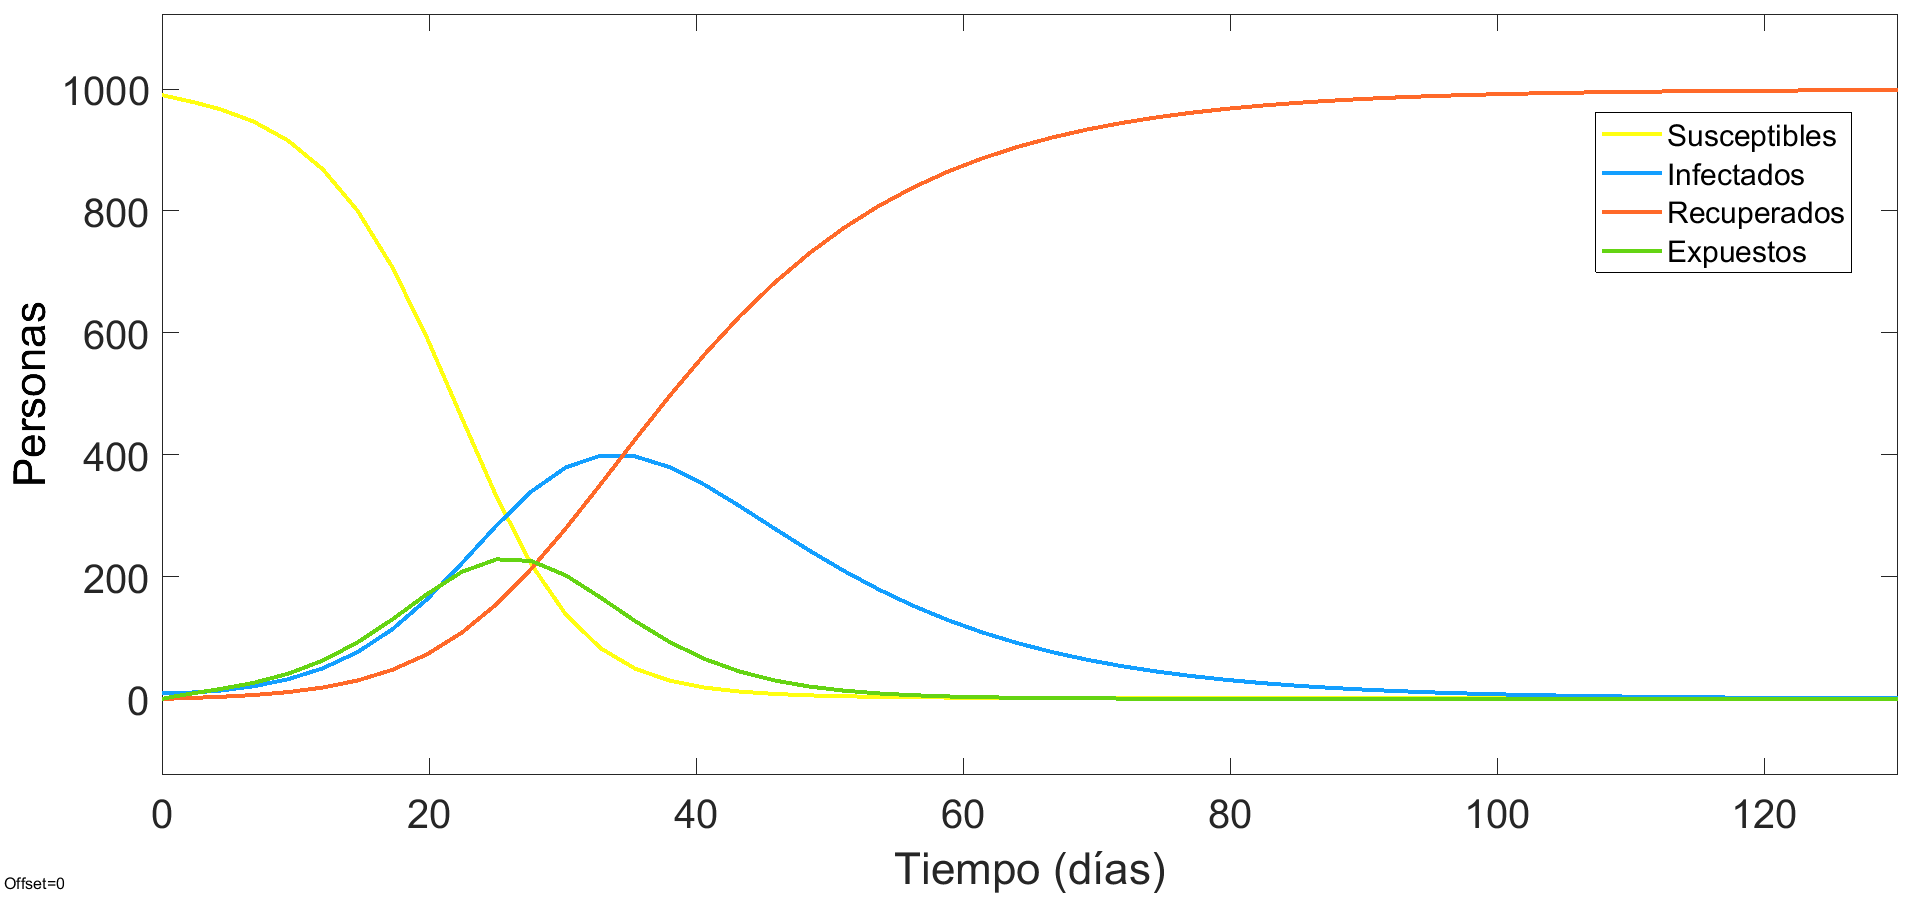
\includegraphics[width=0.7\textwidth]{img/modelo_SEIR_resultado_ejemplo.png}
    \caption{Resultado típico de un modelo SEIR}
    \label{fig:eje SEIR}
    \vspace{0.5cm} % Ajusta el espacio vertical entre la imagen y el texto
\end{figure}

Como se observa en la figura al inicio de la epidemia, casi toda la población son susceptibles, por lo que existe un alto riesgo de contagio. A medida que los individuos susceptibles entran en contacto con personas infecciosas, se infectan y pasan al compartimento de expuestos, lo que hace que el número de susceptibles disminuya rápidamente en las fases iniciales del brote.

El número de expuestos comienza siendo cero, pero crece rápido conforme se producen nuevos contagios. Estas personas están infectadas, pero aún no son contagiosas debido al período de incubación. Una vez transcurrido ese tiempo, pasan al compartimento de infectados. Por esta razón, la curva de los expuestos alcanza su pico antes que la de los infectados. Conforme los expuestos van pasando a infectados, la curva de expuestos disminuye.

La población infectada aumenta a medida que los expuestos se vuelven infecciosos. El número de infectados alcanza su máximo cuando el ritmo de nuevos contagios supera al de las recuperaciones, lo que suele coincidir con el momento en que el número de susceptibles todavía es elevado. A medida que los infectados se recuperan, el número de personas en este compartimento comienza a descender.

Finalmente, el compartimento de recuperados incrementa a medida que los infectados superan la enfermedad y adquieren inmunidad permanente. Esta curva se estabiliza cuando la mayoría de la población ha pasado ya por la enfermedad, indicando el fin de la epidemia.
Importante calcular el número básico de reproducción con estos parámetros \eqref{eq:R0_calculo_7}.
\begin{equation}
R_0 = \frac{\beta}{\gamma} = \frac{0.5}{0.071} \approx 7
\label{eq:R0_calculo_7}
\end{equation}
$R_0$ es 7, con lo que es mayor que 1, por lo tanto la enfermedad tiende a crecer, se ve que en la gráfica \ref{fig:eje SEIR} se cumple este comportamiento.

\subsection{Mejora modelo SEIR}
Mejorar el modelo SEIR como medida de control, incorporando el explícitamente el efecto de la vacunación. Esta adaptación del modelo clásico SEIR se conoce como modelo \textbf{SEIRV} (Susceptibles – Expuestos – Infectados – Recuperados – Vacunados), en el cual se añade un nuevo compartimento denominado V (Vacunados), que permite representar a las personas que, siendo inicialmente susceptibles, reciben una vacuna eficaz y desarrollan inmunidad contra el virus.

En esta versión extendida del modelo, se considera que las personas susceptibles pueden seguir el curso natural de exposición e infección o, alternativamente, pasar directamente al grupo de inmunizados mediante vacunación, uniéndose al compartimento de recuperados, bajo el supuesto de que la inmunidad inducida por la vacuna es completa y duradera, al igual que en el caso de los individuos que se recuperan de la enfermedad. Aunque en la realidad la duración de la inmunidad puede variar y algunas vacunas no garantizan protección absoluta, esta simplificación permite estudiar de forma clara el efecto global de la inmunización sobre la propagación del virus.

Se muestra una representación esquemática del modelo SIS mediante el diagrama de flujo, representado en la figura \ref{fig:eje SEIRV}.

\begin{figure}[H]
    \centering
    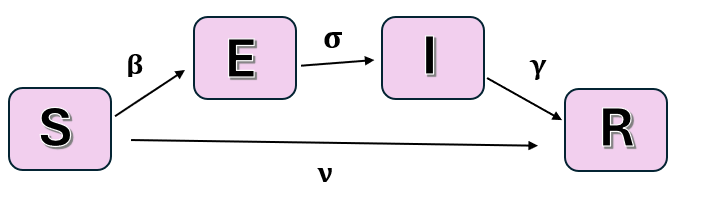
\includegraphics[width=0.7\textwidth]{img/diagrama_SEIRV.png}
    \caption{Diagrama de flujo del modelo SEIRV}
    \label{fig:eje SEIRV}
    \vspace{0.5cm} % Ajusta el espacio vertical entre la imagen y el texto
\end{figure}
También se puede representar el modelo mediante el siguiente sistema de ecuaciones diferenciales \eqref{eq:dS_vacunacion}\eqref{eq:dE_SEIRV}\eqref{eq:dI_SEIRV}\eqref{eq:dR_vacunacion}.
\begin{align}
\frac{dS}{dt} &= -\beta SI - \nu S \label{eq:dS_vacunacion} \\
\frac{dE}{dt} &= \beta SI - \sigma E \label{eq:dE_SEIRV} \\
\frac{dI}{dt} &= \sigma E - \gamma I \label{eq:dI_SEIRV} \\
\frac{dR}{dt} &= \gamma I + \nu S \label{eq:dR_vacunacion}
\end{align}
Donde:
\begin{itemize}
    \item 	La ecuación dS⁄dt \eqref{eq:dS_vacunacion} representa la disminución de personas susceptibles con el tiempo. Este número disminuye por dos mecanismos el contagio y la vacunación. Por contagio cuando los susceptibles entran en contacto con infectados, se infectan y dejan de ser susceptibles. La vacunación los susceptibles salen del compartimento al ponerse la vacuna, ganando inmunidad directa sin tener que pasar por la enfermedad.
    \item 	La ecuación dE⁄dt \eqref{eq:dE_SEIRV} muestra el aumento de personas expuestas, personas infectadas que todavía no son contagiosas, debido a nuevos contagios, y su disminución a medida que pasan a estado de infectados. Aumentan por el término de contagio y disminuyen por el paso a infectados.
    \item 	La ecuación dI⁄dt \eqref{eq:dI_SEIRV}indica la variación del número de personas infectadas. Aumenta a medida que los expuestos se vuelven infecciosos y disminuye cuando los infectados se recuperan. Este balance determina su el número de infectados aumenta produciéndose una epidemia, o si por el contrario disminuye y se controla.
    \item La ecuación dR⁄dt \eqref{eq:dR_vacunacion}, muestra el aumento del número de personas inmunizadas. Se suman tanto los infectados que se recuperan como los susceptibles que se vacunan.
    \item 	Beta ($\beta$), tasa de transmisión: representa cuantos contagios ocurren por unidad de tiempo cuando una personas susceptible entra en contacto con una infectada.
    \item Sigma ($\sigma$), tasa de incubación. Inverso del tiempo de incubación.
    \item Gamma ($\sigma$), tasa de recuperación: inverso del tiempo de recuperación.
    \item 	Nu ($\nu$), tasa de vacunación: representa la fracción de la población susceptible que se vacuna por unidad de tiempo.
\end{itemize}

En este modelo no se ha incluido un compartimento explícito para los vacunados, ya que se asume que la vacunación proporciona una inmunidad equivalente a la adquirida tras pasar la enfermedad. Por lo tanto, las personas vacunadas son incorporadas de manera directa al compartimento de recuperados, simplificando así el modelo sin perder su capacidad explicativa. También dejar claro que no se añade la población total de forma explícita para su simplificación. Se redefine el parámetro beta como ya se ha visto anteriormente.

Es importante señalar que la tasa de transmisión ($\beta$) no varía directamente como consecuencia de la vacunación, ya que se trata de un parámetro biológico y social que describe la probabilidad de contagio efectivo entre un individuo susceptible y uno infectado por unidad de tiempo. Esta tasa depende de factores como la contagiosidad del virus, el número medio de contactos diarios entre personas y las medidas de comportamiento social.

Por tanto, $\beta$ se mantiene constante en el modelo si no cambian ni el virus ni las condiciones sociales de la población. Lo que sí se ve directamente afectado por la vacunación es el número de susceptibles. Al disminuir el tamaño del grupo susceptible mediante la inmunización, también se reduce la probabilidad de que se produzcan nuevos contagios, incluso si $\beta$ permanece constante. Aunque el virus mantenga su capacidad de contagio, al haber menos personas expuestas, disminuye el número efectivo de nuevas infecciones.

Además, se está utilizando la $\beta$ efectiva o ajustada, que es el valor de $\beta$ dividido entre la población total. En este caso, si la población total cambia, el valor de $\beta$ ajustada también cambiará, incluso si $\beta$ se mantiene constante. Esto se debe a que el tamaño poblacional afecta directamente al cálculo del número esperado de contactos efectivos entre susceptibles e infectados.
















\section{Descripción de los datos}
Para cada uno de los modelos estudiados se ha seleccionado una enfermedad cuya dinámica se ajusta adecuadamente a la estructura del modelo. A continuación, se presentan los datos utilizados y se justifica la elección de cada enfermedad en función de las características del modelo correspondiente.

\subsection{Datos modelo SI}
El modelo SI es adecuado para representar enfermedades infecciosas crónicas como el VIH/SIDA, en las que la persona, una vez contagiada, permanece infectada de por vida y no se recupera ni adquiere inmunidad.

En este modelo, la población se divide en dos grupos: susceptibles e infectados, sin contemplar la recuperación. Esto se ajusta bien al comportamiento del VIH, ya que, aunque el virus puede controlarse mediante tratamiento, no se elimina del organismo, y la persona no regresa al estado susceptible ni pasa a un estado de recuperación.

Por tanto, el modelo SI ofrece una herramienta útil para analizar la propagación del VIH y entender cómo evoluciona en función de parámetros como la tasa de transmisión ($\beta$). 
Se va a estudiar la enfermedad en la región MENA\footnote{Oriente Medio y Norte de África}, cuya población total se estima en aproximadamente 400 millones de personas. En cuanto a las personas infectadas con VIH es de alrededor de 240000 personas \cite{Khorrami2023}.

La tasa de transmisión para esta enfermedad es de 0,105 \cite{shakiba2021epidemiological}. Sin embargo, para utilizarlo correctamente es necesario ajustar la beta, para facilitar las ecuaciones no se ha metido la población total, por eso hay que ajustar beta como se muestra en la ecuación \eqref{eq:beta_efectiva2}.
\begin{equation}
\beta_{\text{efectiva}} = \frac{\beta}{N} = \frac{0.105}{400\,000\,000} = 2.625 \times 10^{-10}
\label{eq:beta_efectiva2}
\end{equation}

Lo que significa que cada personas infectada contagia al 0. 00000002625\% de la población susceptible por día.

\subsection{Datos modelo SIS}
La gonorrea constituye un ejemplo representativo de enfermedad infecciosa que se ajusta de forma adecuada al modelo SIS. Este modelo divide a la población en dos compartimentos: susceptibles e infectados. A diferencia de otros modelos que contemplan inmunidad tras la recuperación, en este modelo los individuos, una vez curados, vuelven a ser susceptibles, lo que refleja la dinámica de enfermedades que no generan inmunidad permanente.

En el caso de la gonorrea, una infección de transmisión sexual causada por la bacteria \textit{Neisseria gonorrhoeae}, los individuos infectados pueden recibir tratamiento y curarse, pero no adquieren inmunidad duradera, por lo que, si vuelven a exponerse al patógeno, pueden infectarse de nuevo. Esto implica que una persona puede sufrir múltiples episodios de infección a lo largo de su vida, especialmente si mantiene prácticas sexuales de riesgo o no se siguen medidas preventivas adecuadas.

Como no se genera inmunidad, el equilibrio del sistema se alcanza cuando el número de nuevos contagios se compensa con el número de recuperaciones, manteniéndose una proporción constante de infectados en la población, puede darse una situación de endemicidad.

Por tanto, la gonorrea es un claro ejemplo de cómo una enfermedad puede persistir en una población mediante el mecanismo de reinfección continua, y cómo el modelo SIS resulta útil para analizar su evolución y proponer estrategias de control.

Se ha tomado como referencia la situación epidemiológica en Estados Unidos durante el 2019. En ese año, la población total del país era aproximadamente 328 millones de personas, en cuanto a los casos de personas infectadas ascendía a 1603473 personas \cite{pollock2023estimated}.

La tasa de la enfermedad pude variar en función del comportamiento social, el uso de métodos de protección y otros factores. Pero para este estudio se ha estimado una tasa de 0.25, hay que calcular la beta efectiva \eqref{eq:beta_efectiva}.
\begin{equation}
\beta_{\text{efectiva}} = \frac{\beta}{N} = \frac{0.25}{328\,000\,000} = 7 \times 10^{-10}
\label{eq:beta_efectiva}
\end{equation}



Respecto a la tasa de recuperación, se considera que, en un país con un sistema sanitario desarrollado como Estados Unidos, los individuos infectados reciben tratamiento de forma relativamente rápida. Aunque sin tratamiento la infección puede durar semanas o incluso meses, con tratamiento, el tiempo medio de recuperación se estima en unos 7 días. Por lo tanto, la tasa de recuperación se calcula como se oberva en \eqref{eq:gamma}.

\begin{equation}
\gamma = \frac{1}{\text{tiempo de recuperación}} = \frac{1}{7}
\label{eq:gamma}
\end{equation}

\subsection{Datos modelo SIR}
El sarampión es una enfermedad vírica altamente contagiosa que se ajusta adecuadamente a los supuestos y estructura de este modelo. El modelo SIR se utiliza para representar enfermedades en las que los individuos, una vez recuperados, desarrollan inmunidad permanente. Este es precisamente el caso del sarampión, tras superar la infección, el sistema inmunológico genera una respuesta eficaz que protege de por vida frente a futuros contagios.

Además, el sarampión presenta una transmisión rápida y eficiente dentro de poblaciones susceptibles. Su número básico de reproducción es muy alto, por lo que, en ausencia de inmunización, una sola persona infectada puede contagiar a muchas otras en un entorno sin protección.

Otra característica que lo hace idóneo para este modelo es que el sarampión tiene un periodo de infección claramente definido, durante el cual los individuos pueden transmitir la enfermedad antes de recuperarse. Esto permite representar su dinámica mediante las ecuaciones del modelo SIR, donde los individuos pasan de ser susceptibles a infectados, y finalmente a recuperados sin posibilidad de reinfección.

El hecho de que el sarampión haya sido históricamente una enfermedad que se propagaba en oleadas epidémicas , especialmente antes de la introducción de la vacuna, lo convierte en un buen ejemplo para el estudio de brotes mediante modelos matemáticos como el SIR. Incluso actualmente, cuando los niveles de vacunación disminuyen en ciertas regiones, se pueden observar rebrotes cuya dinámica encaja con las predicciones de este tipo de modelos.

Por tanto, el sarampión reúne todas las condiciones necesarias para ser modelado con un enfoque SIR transmisión rápida y eficiente, ausencia de reinfección tras recuperación, periodo infeccioso finito y bien definido, y potencial para generar epidemias si no se controla. 

Se ha elegido analizar la propagación del sarampión en Estados Unidos antes de la introducción de la vacuna en 1963. El país contaba con una población de aproximadamente 189 millones de personas \cite{datosmacro_usa_1963}, mientras que se registraban alrededor de 500 mil casos anuales. Datos que reflejan la alta incidencia del sarampión.
Uno de los parámetros más relevantes para modelar esta enfermedad es el número básico de reproducción, que representa el número medio de personas susceptibles que puede llegar a contagiar un solo individuo infectado en una población completamente susceptible. En el caso del sarampión, este valor es excepcionalmente alto, estimándose en torno a $R_0$ = 12 \cite{solomon2019peter}. Significa que, en ausencia de medidas de control, cada persona infectada podría contagiar a doce individuos, lo que explica su elevada transmisibilidad y su capacidad para provocar grandes brotes epidémicos.

Además, se conoce que el tiempo de recuperación de la enfermedad es de 14 días \cite{ops_sarampion}. Esto implica que la tasa de recuperación (~$\gamma$) se calcula en la ecuación \eqref{eq:gamma_14}
\begin{equation}
\gamma = \frac{1}{\text{tiempo medio de recuperación}} = \frac{1}{14} = 0{,}071 \,\text{días}^{-1}
\label{eq:gamma_14}
\end{equation}

Dado que la relación entre $R_0$, beta y gamma viene dada por la fórmula \eqref{eq:R0}
\begin{equation}
R_0 = \frac{\beta}{\gamma}
\label{eq:R0}
\end{equation}

Se despeja beta para poder calcular la tasa de transmisión \eqref{eq:beta_calculo}
\begin{equation}
\beta = R_0 \times \gamma = 12 \times 0{,}071 = 0{,}852
\label{eq:beta_calculo}
\end{equation}

Una vez se ha calculado beta\eqref{eq:beta_calculo}, hay que calcular la beta ajustada para este modelo, es decir, la beta efectiva \eqref{eq:beta_efectiva2}
\begin{equation}
\beta_{\text{efectiva}} = \frac{\beta}{N} = \frac{0{,}852}{189\,000\,000} = 4{,}5 \times 10^{-9}
\label{eq:beta_efectiva2}
\end{equation}

Lo que significa que cada personas infectado contagia al 0.00000045\% de la población susceptible por día.

\vspace{2em}
\textbf{Modelo SIRV}. La única diferencia introducida es la incorporación de una tasa de vacunación correspondiente a una cobertura del 92,7\% de la población en un periodo de seis meses, lo cual se ajusta a datos reales observados en campañas de vacunación contra el sarampión. Este porcentaje se ha convertido en un valor de tasa ($\nu$) para integrarlo dentro del sistema de ecuaciones del modelo SIRV, y así simular cómo evolucionaría la epidemia bajo una estrategia de inmunización masiva \cite{cdc_measles_cases_2025}.

De esta manera, se busca evaluar cuantitativamente cómo la vacunación modifica la evolución del brote, en particular en términos de reducción de contagios y aceleración de la inmunidad colectiva, y contrastar estos resultados con los obtenidos previamente en ausencia de intervenciones.
Se tiene la cobertura de vacunación, pero hay que calcular la tasa de vacunación con los datos que se han obtenido. Se calcula a partir de la siguiente fórmula \eqref{eq:nu_vacunacion}. 
\begin{equation}
\nu = \frac{-\ln(1 - 0{,}927)}{183} \approx 0{,}014
\label{eq:nu_vacunacion}
\end{equation}
Esto significa que aproximadamente el 1,4\% de la población susceptible se vacuna cada día durante ese periodo, adquiriendo inmunidad y pasando directamente al compartimento de recuperados. Esta tasa se incorpora en el modelo como un nuevo flujo desde susceptibles a recuperados, simulando el efecto de la vacunación masiva sobre la dinámica de propagación del sarampión.


\subsection{Datos modelo SEIR}
Para la implementación del modelo SEIR con datos reales se ha seleccionado la enfermedad del COVID-19. Esta elección se debe a que las características epidemiológicas del COVID-19 se ajustan a la estructura del modelo, lo que permite representar de forma realista su dinámica de transmisión.

Una de las principales razones por las que el modelo SEIR es adecuado para esta enfermedad es la presencia de un periodo de incubación bien definido. Durante este intervalo, las personas infectadas no presentan síntomas clínicos y, en la mayoría de los casos, no son aún contagiosas. Esta fase de latencia es un aspecto clave que el modelo SEIR incorpora a través del compartimento de expuestos, que representa a los individuos infectados que aún no han desarrollado la capacidad de transmitir el virus.

Tras este periodo, los individuos entran en la fase de infectados, en la cual sí pueden contagiar a otras personas. Esta fase incluye tanto a los casos sintomáticos como a los asintomáticos. 

Posteriormente, los individuos pasan al estado de recuperados tras superar la infección. Las personas adquieren inmunidad frente al virus. Aunque existen evidencias de que esta inmunidad puede no ser permanente, especialmente en presencia de variantes del virus, durante un tiempo actúa como barrera frente a nuevos contagios. Este comportamiento también puede modelarse en versiones extendidas del SEIR que incluyen pérdida de inmunidad, pero en un enfoque básico, la recuperación con inmunidad justifica la inclusión del compartimento recuperados.

En resumen, la COVID-19 reúne las condiciones esenciales para que su propagación pueda ser estudiada eficazmente mediante un modelo SEIR presenta un periodo de incubación con latencia infecciosa, se transmite entre personas por contacto directo o por vía aérea, y tras la infección, los individuos desarrollan una cierta inmunidad.

Gracias a esta correspondencia entre las fases clínicas de la enfermedad y los compartimentos del modelo, el uso del modelo SEIR no solo permite analizar la evolución teórica del brote, sino también simular diferentes escenarios de control, evaluar medidas de contención y estimar la carga sanitaria a lo largo del tiempo. 

Se ha elegido como caso de estudio la evolución de la COVID-19 en España, desde la aparición del primer caso confirmado, registrado el 31 de enero de 2020 \cite{primer_caso_covid_espana}. Desde esa fecha hasta el 28 de diciembre de 2020 a las 14:00 horas, se notificaron oficialmente un total de 1879413 casos acumulados de personas infectadas por SARS-CoV-2 \cite{sanidad_covid_situacion}. En ese mismo año, la población total de España era de aproximadamente 47370000 habitantes \cite{datacommons_espana_demografia}.

En las primeras fases de la pandemia, el número básico de reproducción del virus SARS-CoV-2 se situaba, según estimaciones epidemiológicas, entre 2 y 3 \cite{garcia_r0_desescalada}. Esto indica que cada persona infectada transmitía el virus entre 2 y 3 personas, lo que implica una tendencia clara al crecimiento exponencial del brote en ausencia de medidas de control o inmunidad previa en la población.

En cuanto a los parámetros clínicos de la enfermedad, el periodo de incubación, entendido como el intervalo desde la exposición al virus hasta el momento en que el individuo se vuelve contagioso, se estima con una media de 5.4 días \cite{lauer2020incubation}. Hay que calcular la tasa de incubación ($\sigma$)\eqref{eq:sigma}
\begin{equation}
\sigma = \frac{1}{\text{tiempo de incubación}} = \frac{1}{5{,}4} = 0{,}185
\label{eq:sigma}
\end{equation}

Por otro lado, el tiempo medio de recuperación depende de la gravedad del cuadro clínico. En los casos leves, suele rondar las 2 semanas, mientras que en los casos moderados o graves puede extenderse entre 3 y 6 semanas. Para simplificar el análisis y mantener la coherencia en el modelo, se considerará un tiempo medio de recuperación de 14 días \cite{ada_duracion_covid}. Hay que calcular la tasa de recuperación \eqref{eq:gamma_7}
\begin{equation}
\gamma = \frac{1}{\text{tiempo medio de recuperación}} = \frac{1}{14} = 0{,}071 \,\text{días}^{-1}
\label{eq:gamma_7}
\end{equation}

Para finalizar, hay que calcular la tasa de transmisión, para ello utilizamos el $R_0$, ya que relaciona la gamma y beta. Se aplica la fórmula del $R_0$. Se va a optar por utilizar el valor de $R_0$ = 3, ya que es un escenario más desfavorable y representativo, es más contagioso. La ecuacion \eqref{eq:R0} se utiliza para calcular beta.\eqref{eq:beta_R0_gamma}
\begin{equation}
\beta = R_0 \times \gamma = 3 \times 0{,}071 = 0{,}213
\label{eq:beta_R0_gamma}
\end{equation}

Una vez se ha calculado la beta, hay que calcular la beta efectiva\eqref{eq:beta_efectiva_final}.
\begin{equation}
\beta_{\text{efectiva}} = \frac{\beta}{N} = \frac{0{,}213}{47\,370\,000} \approx 4{,}5 \times 10^{-9}
\label{eq:beta_efectiva_final}
\end{equation}

\vspace{2em}


\textbf{Modelo SEIRV}. Con el fin de ampliar el análisis realizado sobre el COVID-19 mediante el modelo SEIR, se ha decidido incorporar la vacunación en la simulación a través del modelo SEIRV. Permite estudiar cómo una campaña de vacunación influye en la dinámica de propagación del virus, proporcionando una visión más realista del contexto epidemiológico vivido en España durante la pandemia.
Para mantener la coherencia entre escenarios, se han conservado los mismos parámetros epidemiológicos utilizados en el modelo SEIR básico: la tasa de transmisión, el tiempo de incubación y la tasa de recuperación. La diferencia es la inclusión de un parámetro, la tasa de vacunación, que representa el efecto de la inmunización masiva iniciada en España a finales de 2020.
Según los datos oficiales, la campaña de vacunación comenzó el 27 de diciembre de 2020, y hasta el 15 de enero de 2021 se habían administrado 768.950 dosis \cite{sanidad_giv_20210115}. Posteriormente, la cobertura vacunal alcanzó el 92,6\% de la población en un año \cite{sanidad_historico_covid}. Para incorporar esta información en el modelo, es necesario calcular la tasa diaria de vacunación, lo cual se realiza con la siguiente fórmula \eqref{eq:nu_926}.
\begin{equation}
\nu = \frac{-\ln(1 - 0{,}926)}{365} \approx 0{,}0071
\label{eq:nu_926}
\end{equation}

Este valor indica que aproximadamente el 0,71\% de la población susceptible se vacuna cada día durante ese periodo. En el modelo, estas personas abandonan directamente el compartimento de susceptibles y pasan al de recuperados, ya que se considera que la vacunación confiere una inmunidad funcional equivalente a la adquirida tras superar la infección.
Se mantiene, la misma estructura conceptual del modelo SEIR. La única diferencia es la inclusión del flujo adicional introducido por la vacunación. Así, el modelo SEIRV permite simular con mayor precisión cómo las campañas de inmunización modifican la evolución de la pandemia, en particular reduciendo el número de contagios y acelerando el logro de la inmunidad colectiva.






\section{Técnicas y herramientas}

\subsection{MATLAB}
\texttt{MATLAB} (acrónimo de MATrix LABoratory) \cite{mathworks_matlab} es una plataforma de programación y entorno de cálculo numérico desarrollada por MathWorks, diseñada para facilitar el análisis de datos, la creación de modelos matemáticos y el desarrollo de algoritmos. Gracias a su estructura basada en matrices y a su sintaxis intuitiva, permite realizar cálculos complejos y procesar grandes volúmenes de datos de forma eficiente. Su lenguaje de programación está optimizado para operaciones matemáticas, lo que lo hace más accesible que lenguajes tradicionales para tareas de análisis técnico.

El entorno incluye un completo IDE\footnote{Entorno de desarrollo integrado} que proporciona herramientas para la edición de código, visualización de datos, depuración y creación de interfaces gráficas. Además, cuenta con una amplia colección de toolboxes\footnote{Paquetes de herramientas adicionales} diseñados para áreas como el procesamiento de señales, control automático, aprendizaje automático o simulación de sistemas dinámicos.

\texttt{MATLAB} está disponible para los principales sistemas operativos. Su uso está extendido tanto en industria como en el ámbito académico, gracias a su versatilidad, documentación extensa y soporte técnico especializado. En entornos universitarios, su acceso suele estar facilitado mediante licencias institucionales, lo que permite a estudiantes y docentes utilizar todas sus funcionalidades sin coste adicional.

Aunque existen alternativas de código abierto , \texttt{MATLAB} se mantiene como una herramienta de referencia debido a su estabilidad, potencia en el tratamiento de datos numéricos y facilidad de uso, especialmente en tareas relacionadas con la ingeniería, las matemáticas aplicadas y las ciencias físicas.

\subsection{Simulink}
\texttt{Simulink} \cite{mathworks_simulink} es un entorno de simulación y diseño basado en diagramas de bloques, desarrollado por MathWorks e integrado de en \texttt{MATLAB}. Está orientado al modelado, simulación y análisis de sistemas dinámicos multidominio, que permite representar y estudiar el comportamiento de sistemas complejos mediante bloques funcionales interconectados. Gracias a su enfoque gráfico, \texttt{Simulink} facilita el desarrollo de modelos intuitivos y modulares sin necesidad de escribir código manual, aunque permite combinarlo con scripts de \texttt{MATLAB} para ampliar su funcionalidad.

\texttt{Simulink} se utiliza ampliamente en campos como el control automático, la electrónica, la ingeniería de comunicaciones, la automoción, la robótica, entre otros. Permite modelar sistemas en tiempo continuo, tiempo discreto o híbridos, incluyendo componentes físicos, señales lógicas, redes de control, sistemas mecánicos, eléctricos o térmicos. Su integración con toolboxes específicos amplía sus capacidades para abordar el modelado físico, la lógica de eventos o la optimización de controladores.

Una de las principales ventajas de \texttt{Simulink} es su capacidad de realizar una simulación previa a la implementación, permitiendo validar el comportamiento del sistema antes de llevarlo a hardware real. Además, ofrece herramientas avanzadas para el análisis de rendimiento, depuración de modelos, generación automática de código en C/C++ o HDL y conexión con sistemas de tiempo real.

En el ámbito académico, \texttt{Simulink} es una herramienta clave para enseñar conceptos de sistemas dinámicos, control y simulación, ya que su interfaz visual mejora la comprensión conceptual y reduce la curva de aprendizaje. Al igual que \texttt{MATLAB}, está disponible en muchas universidades mediante licencias académicas, lo que facilita su uso en proyectos de investigación, desarrollo y trabajos de fin de grado.

\subsection{App Desinger}
\texttt{App Designer} \cite{mathworks_matlab} es una herramienta integrada en \texttt{MATLAB} que permite crear aplicaciones interactivas con GUIs\footnote{Interfaces gráficas de usuario} de forma visual e intuitiva. Está diseñada para facilitar el desarrollo de aplicaciones profesionales, combinando un entorno de diseño gráfico de componentes (botones, gráficos, deslizadores, tablas, etc.) con un editor de código basado en el lenguaje de \texttt{MATLAB}.

A diferencia de herramientas anteriores como \texttt{GUIDE}, \texttt{App Designer} ofrece una experiencia más moderna, con mayor integración, organización del código orientado a objetos, y funcionalidades avanzadas para el desarrollo de interfaces. Las aplicaciones creadas pueden ejecutarse directamente desde \texttt{MATLAB} o compartirse como aplicaciones independientes.

Esta herramienta es especialmente útil para prototipar algoritmos, visualizar datos de forma dinámica o crear herramientas personalizadas para usuarios finales, sin necesidad de conocimientos profundos en lenguajes de programación externos.

\subsection{LaTeX}
\texttt{LaTeX} \cite{latexproject} es un sistema de composición de textos de alta calidad, especialmente diseñado para la creación de documentos científicos y técnicos que requieren la presentación precisa de fórmulas matemáticas, gráficos y referencias bibliográficas. Debido a su potencia y flexibilidad, \texttt{LaTeX} es el estándar en la academia para la elaboración de informes, tesis y artículos científicos.

Para facilitar el trabajo colaborativo y la edición, se utilizó \texttt{Overleaf}, una plataforma en línea que permite editar, compilar y gestionar documentos \texttt{LaTeX} directamente desde el navegador web, sin necesidad de instalar software adicional. \texttt{Overleaf} también ofrece integración con sistemas de control de versiones y plantillas personalizadas, lo que mejora la organización y la eficiencia en la elaboración del documento.

\subsection{GitHub}
\texttt{GitHub} \cite{githubdocs} es una plataforma de desarrollo colaborativo que permite alojar, gestionar y controlar versiones de proyectos mediante el sistema de control de versiones \texttt{Git}. Su uso facilita el seguimiento del progreso del proyecto, el almacenamiento seguro del código y la colaboración entre múltiples desarrolladores.

En este proyecto, \texttt{GitHub} se ha utilizado como herramienta de control de versiones y respaldo del código fuente, incluyendo los modelos en \texttt{Simulink}, el desarrollo de la aplicación en \texttt{App Designer} y los documentos en \texttt{LaTeX}. Gracias a esta plataforma, ha sido posible mantener un historial detallado de los cambios realizados, identificar errores, volver a versiones anteriores del proyecto cuando ha sido necesario y garantizar una mayor organización y trazabilidad durante el desarrollo.

Además, al ser una plataforma en la nube, \texttt{GitHub} ha permitido trabajar desde diferentes dispositivos sin necesidad de configurar repositorios locales complejos, y ha servido como medio para compartir el proyecto en caso de ser necesario.

